\section{Fine Tuning Speech Recognition on Model Predictions}

This section details an improved approach for training a silent speech
recognition system by pre-training a DeepSpeech2 model directly on the
predictions of a chosen portion of the dataset.

This is better than performing
speech recognition on the final waveform generated in the Digital Voicing
(\cite{gaddy2020digital}) paper.

Although the method used in that paper isn'\t
used directly for speech recognition, the end-to-end evaluation procedure
can be used for speech recognition by transducing from from the silent EMG
data into speech features, then using a vocoder to go from speech features
into an audio waveform and then using a pretrained ASR model to predict speech
from the waveform.

This proposed method skips over the vocoder entirely which improves the
end-to-end performance as there is now one less step involved whilst
also requiring far less training data, and therefore training time,
for the entire silent speech recognition pipeline.

\subsection{Related Work}

The intuition behind fine tuning a speech recognition model on the
predicted mel spectrograms from the transduction model comes
from the literature for speech recognition. Typical speech recognition models
suffer from a loss of accuracy when they are only trained on clean audio data
and then evaluated on a noisy dataset (\cite{DS2_original}). For example,
in the DeepSpeech2 paper the authors trained their speech recongition
model on different fractions of a dataset.

Their results showed that the
performance of a model trained on a clean dataset, when evaluated on a dataset
of clean audio compared to noisy audio, showed a larger gap when trained on less
data. When the authors trained their model on 1\% of the entire dataset (120 hours),
the WER for the clean dataset was 29.23\% whereas for the noisy dataset it was 50.97\%.
However when they trained on the full dataset (12,000 hours), the clean audio
WER was 8.46\% compared to 13.59\% for the noisy dataset.

The results from their paper show a strong relationship between datasize and
affect on evaluation performance on a noisy dataset. For this reason, this paper
researches the affect of providing predicted speech from the SOTA silent speech
transduction model to a speech recognition model to close the gap between
the WER when evaluted on the ground truth audio features and the predicted
audio features (\cite{DS2_original}).

\iffalse
\subsection{Relevance to EMG Silent Speech Classification}

This issue is also reflected in the transduction task. The state-of-the-art
transduction model within the second David Gaddy (\cite{gaddy2021improved}) paper
will always produce audio outputs with artefacts because of the final vocoder layer
and because the mel spectrograms will always at best be an approximation.

This becomes problematic if you want to use the transduction model as a basis for a
speech recognition system as most pre-trained speech recognition systems
are trained on clean audio datasets which means that naively applying a speech
recognition system on top of the transduction model will result in reduced performance.
\fi

\subsection{Relation to EMG Silent Speech Classification}

\begin{figure}
  \centering
  \begin{subfigure}{.5\textwidth}
    \centering
    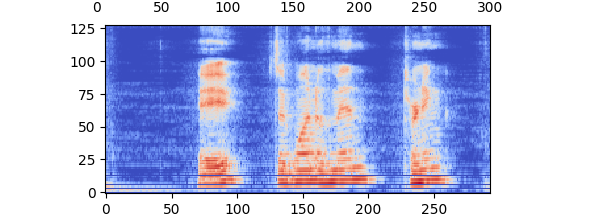
\includegraphics[width=1.\linewidth]{graphics/mel_vs_pred/ideal/458_g.png}
    \caption{Ground Truth Mel Spectrogram}
    \label{fig:sub1}
  \end{subfigure}%
  \begin{subfigure}{.5\textwidth}
    \centering
    \includegraphics[width=1\linewidth]{graphics/mel_vs_pred/ideal/458_p.png}
    \caption{Predicted Mel Spectrogram}
    \label{fig:sub2}
  \end{subfigure}
  \caption{Comparison of Ideal Ground Truth and Predicted Mel Spectrograms}
  \label{fig:ideal-gt-vs-pred-mel}
  From both of these mel spectrograms, we can see the low level features
  of the predicted mel spectrogram appear blurrier (the horizontal red lines
  with blurry edges).
  Not pictured in the figures, is
  the text transcription for the utterances which is: '"Eh?" said one of the men, turning.'.
\end{figure}

\subsection{Proposed Method}

My proposed method involves pre-training the state-of-the-art EMG silent speech
transduction model from the second Digital Voicing paper (\cite{gaddy2021improved}),
and then saving the predicted mel spectrogram speech features from the model as a
custom dataset. Then this dataset will be used along with the ground truth audio
files to train a regular speech recognition model. Based on my literature review
and intuition from exploring the audio outputs viewing the mel spectrogram
visulisations from the model, I was confident this approach would be successful.

\subsection{Research Question}

\subsection{Hypothesis}

My hypothesis based on my literature review, 

\iffalse
However this also opens up a new possibility, use the error correcting properties
of speech recognition systems to improve the synthesis of speech.
\fi

\subsection{Closed Vocabulary Dataset}

The closed vocabulary dataset is the first dataset used to determine how much better
a speech recognition model can be improved by training on the predicted mel spectrograms
from an already trained transduction model.

The WER of the closed vocabulary ASR model trained only on the training dataset
of the closed vocab dataset is 37\%. This means that we would not expect the WER
of the model, when it's evaluated on transduced examples, to perform better than
the ground truth word-error rate.

% (Desc.) UoP: FYP: SEMG ASR (Finetune DS2 on Transducer Outputs #8)
{\small\begin{center}
\captionof{table}{DeepSpeech2 Closed Vocab Finetuned Results}
\begin{tabular} {  l  c  c  }
\hline
\textbf{Dataset} & \textbf{CER} & \textbf{WER} \\
\hline
Ground Truth (GT) & 87.10 & 100.50 \\
Voiced & 51.27 & 87.33 \\
Silent & 38.80 & 78.10 \\
Silent, Voiced & \textbf{35.26} & 75.33 \\
\hline
Silent, Voiced, GT & 35.72 & \textbf{70.83} \\
\hline
\end{tabular}
\end{center}}

The above results do not use phonemeic prediction and only use greedy decoding
in the decoder. DeepSpeech2 is also not the SOTA model for speech recognition
which also reduces the performance. This means that the best WER of 70.83\% could
be improved upon a lot more.

For the combined silent, voiced and GT condition, the model is pre-trained on the
ground truth model and and then fine-tuned on the predictions of the
silent and voiced utterances.

Here we can see that training on predictions from both modalities from scratch
is better than training on a single modality only. However the model is only
evaluated on silent EMG text classifications which means that for this experiment,
training on silent and voiced predicted speech improves the performance when
evaluating on only the silent EMG predictions.

This may be because both of the
individual datasets are small (only 400 utterances) so doubling the dataset to
800 utterances gives the model far more examples to learn from, even though the
voiced examples diverge from the silent examples.

\subsection{Open Vocabulary (Parallel-Only) Dataset}

The next dataset used is the parallel voiced and silent EMG data. This is used because
it's smaller than using the entire open vocabulary condition dataset in one go which
makes training the individual ASR models and the transduction model faster.

The WER of the ASR model trained only on the
training dataset of the open vocabulary parallel voiced audio is 64.47\%.

% (Desc.) UoP: FYP: SEMG ASR (Finetune DS2 on Transducer Outputs #8)
{\small\begin{center}
\captionof{table}{DeepSpeech2 Open Vocabulary Parallel Finetuned Results}
\begin{tabular} {  l  c  c  }
\hline
\textbf{Dataset} & \textbf{CER} & \textbf{WER} \\
\hline
Ground Truth (GT) & 66.70 & 110.49 \\
Voiced & 156.29 & 100.00 \\
Silent & 44.21 & 84.19 \\
Silent, Voiced & 42.11 & 85.30 \\
Voiced, GT & 43.06 & 84.65 \\
Silent, GT & 41.24 & 83.97 \\
\hline
Silent, Voiced, GT & \textbf{41.02} & \textbf{81.69} \\
\hline
\end{tabular}
\end{center}}

Due to the results of the closed vocabulary training condition and time constraints,
training on the voiced portion of the open vocabulary paralell mel spectrogram
predictions wasn't conducted.

There is one interesting difference in this training run compared to the closed
vocabulary dataset. Training on the silent EMG and voiced EMG conditions together
reduces performance. This may be because training on both together was better
on training on just the silent EMG signals for the closed vocabulary dataset
because the silent EMG dataset only contained 400 data samples so doubling
the dataset to 800 data samples, even though the vocalised samples are sub-optimal,
is better. However, here the silent EMG dataset is comprised of 2,778 data samples
which means that the difference between the silent EMG and voiced EMG predicted
mel spectrograms is reducing the performance of the ASR model more than having a
larger overall dataset is beneficial.

\subsection{Open Vocabulary Full (Parallel and Non-Parallel) Dataset}

This dataset is the full entire dataset, not including the closed vocabulary
dataset. The experiments for this dataset include the same experiments for
the previous two datasets. However, extra experiments are added for the additional
non-parallel vocal EMG mel spectrogram predictions. The paralell silent and voiced
mel spectrogram predictions are included here to show how predicted speech features
from a model trained with more data improve the predictions of the same dataset.
This has the effect of making the predicted mel spectrograms closer to the ground
truth mel spectrograms which means the model is better able to classify the text
as the dataset for the entire training regime is closer to the same underyling distribution.

The WER for the ground truth model evaluted on the audio is 45\%. This means that we wouldn'\t
expect the model to have a lower WER than this value.

{\small\begin{center}
\captionof{table}{DeepSpeech2 Open Vocabulary Full Dataset Finetuned Results}
\begin{tabular} {  l  c  c  }
\hline
\textbf{Dataset} & \textbf{CER} & \textbf{WER} \\
\hline
Ground Truth (GT) & 61.99 & 100.74 \\
Parallel Voiced & -- & - \\
Silent & - & - \\
Silent, Parallel Voiced & - & - \\
\hline
Silent, Parallel Voiced, GT & 32.48 & \textbf{68.26} \\
Silent, Parallel Voiced, Non-Parallel Voiced, GT & \textbf{31.16} & 68.51 \\
\hline
\end{tabular}
\end{center}}

Here we can see that when the transduction model is trained on the full dataset,
it produces the best final WER. However there is also another interesting finding,
fine tuning the ground truth model on the silent, parallel voiced and non-parallel
voiced harms the overall WER but the CER continues to improve. This means that
the model is better able to predict individual characters but it's ability to
predict words has been slightly reduced.

\subsection{Implementation Errors}

\begin{figure}
  \centering
  \begin{subfigure}{.5\textwidth}
    \centering
    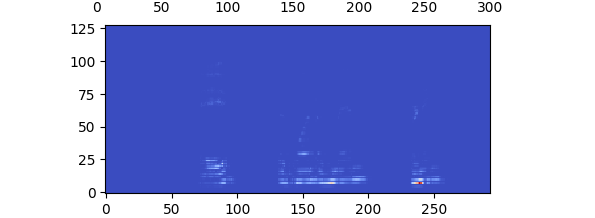
\includegraphics[width=1.\linewidth]{graphics/mel_vs_pred/real/458_g.png}
    \caption{Ground Truth Mel Spectrogram}
    \label{fig:sub1}
  \end{subfigure}%
  \begin{subfigure}{.5\textwidth}
    \centering
    \includegraphics[width=1\linewidth]{graphics/mel_vs_pred/real/458_p.png}
    \caption{Predicted Mel Spectrogram}
    \label{fig:sub2}
  \end{subfigure}
  \caption{Comparison of Real Ground Truth and Predicted Mel Spectrograms}
  \label{fig:real-gt-vs-pred-mel}
  From both of these mel spectrograms, we can see the the low level features
  of the predicted mel spectrogram appear blurrier (the curvy red lines).
  This is because the transduction model a simple linear layer (MLP) between the final
  transformer layer and the output. This limits the ability of the model to produce
  more fine tuned results. Not pictured in the figures, is
  the text transcription for utterances which is: '"Eh?" said one of the men, turning.'.
\end{figure}

One interesting implementation error that was found after conducting the experiments
was that the ground truth audio files have not had the exact same preprocessing techniques
applied as the target mel spectrograms which the transduction model uses as a ground truth
target during training, which can be seen in Figure \ref{fig:real-gt-vs-pred-mel}.

The main difference is that the mel spectrogram values from the transduction model are
log-mel spectrogram values. This is a common preprocessing technique in machine learning
used to make it easier for a regression model to predict a real valued output. This finding
may confound the results for the ground truth results in the above experiments. Interestingly,
training the ASR model on the grouth truth represented as raw mel spectrograms mixed
with the log-mel spectrograms of the transducer predictions together still results in better
performance.

This means that performance of this model may be greatly increased in the future by fixing
this bug. Unfortunately this bug was discovered towards the end of the project where it would
be too time consuming to explore the effect of fixing this bug.

\subsection{Summary}

In summary, this approach proves to be very successful for producing
an efficient EMG silent speech recognition system which can match the
performance of an old transducer model, re-purposed for ASR, while
the speech recognition portion of the new proposed system is only trained
on around 33 hours of data versus 3,817 (\cite{deepspeech0.7.0-training-ref}) of data.